% ========================================
%	Header einbinden
% ========================================

\documentclass[bibtotoc,titlepage]{scrartcl}

% Deutsche Spracheinstellungen
\usepackage[ngerman,german]{babel, varioref}
\usepackage[T1]{fontenc}
\usepackage[utf8]{inputenc}

%\usepackage{marvosym}

\usepackage{amsfonts}
\usepackage{amssymb}
\usepackage{amsmath}
\usepackage{amscd}
\usepackage{amstext}

\usepackage{longtable}

%\usepackage{bibgerm}

\usepackage{footnpag}

\usepackage{ifthen}                 %%% package for conditionals in TeX
\usepackage[amssymb]{SIunits}
%Für textumflossene Bilder und Tablellen
%\usepackage{floatflt} - veraltet

%Für Testzwecke aktivieren, zeigt labels und refs im Text an.
%\usepackage{showkeys}

% Abstand zwischen zwei Absätzen nach DIN (1,5 Zeilen)
% \setlength{\parskip}{1.5ex plus0.5ex minus0.5ex}

% Einrückung am Anfang eines neuen Absatzes nach DIN (keine)
%\setlength{\parindent}{0pt}

% Ränder definieren
% \setlength{\oddsidemargin}{0.3cm}
% \setlength{\textwidth}{15.6cm}

% bessere Bildunterschriften
%\usepackage[center]{caption2}


% Problemlösungen beim Umgang mit Gleitumgebungen
\usepackage{float}

% Nummeriert bis zur Strukturstufe 3 (also <section>, <subsection> und <subsubsection>)
%\setcounter{secnumdepth}{3}

% Führt das Inhaltsverzeichnis bis zur Strukturstufe 3
%\setcounter{tocdepth}{3}
\usepackage[version=3]{mhchem}
	\mhchemoptions{minus-sidebearing-left=0.06em, minus-sidebearing-right=0.11em}
\usepackage{exscale}

\newenvironment{dsm} {\begin{displaymath}} {\end{displaymath}}
\newenvironment{vars} {\begin{center}\scriptsize} {\normalsize \end{center}}


\newcommand {\en} {\varepsilon_0}               % Epsilon-Null aus der Elektrodynamik
\newcommand {\lap} {\; \mathbf{\Delta}}         % Laplace-Operator
\newcommand {\R} { \mathbb{R} }                 % Menge der reellen Zahlen
\newcommand {\e} { \ \mathbf{e} }               % Eulersche Zahl
\renewcommand {\i} { \mathbf{i} }               % komplexe Zahl i
\newcommand {\N} { \mathbb{N} }                 % Menge der nat. Zahlen
\newcommand {\C} { \mathbb{C} }                 % Menge der kompl. Zahlen
\newcommand {\Z} { \mathbb{Z} }                 % Menge der kompl. Zahlen
\newcommand {\limi}[1]{\lim_{#1 \rightarrow \infty}} % Limes unendlich
\newcommand {\sumi}[1]{\sum_{#1=0}^\infty}
\newcommand {\rot} {\; \mathrm{rot} \,}         % Rotation
\newcommand {\grad} {\; \mathrm{grad} \,}       % Gradient
\newcommand {\dive} {\; \mathrm{div} \,}        % Divergenz
\newcommand {\dx} {\; \mathrm{d} }              % Differential d
\newcommand {\cotanh} {\; \mathrm{cotanh} \,}   %Cotangenshyperbolicus
\newcommand {\asinh} {\; \mathrm{areasinh} \,}  %Area-Sinus-Hyp.
\newcommand {\acosh} {\; \mathrm{areacosh} \,}  %Area-Cosinus-H.
\newcommand {\atanh} {\; \mathrm{areatanh} \,}  %Area Tangens-H.
\newcommand {\acoth} {\; \mathrm{areacoth} \,}  % Area-cotangens
\newcommand {\Sp} {\; \mathrm{Sp} \,}
\newcommand {\mbe} {\stackrel{\text{!}}{=}}     %Must Be Equal
\newcommand{\qed} { \hfill $\square$\\}
\renewcommand{\i} {\imath}
\def\captionsngerman{\def\figurename{\textbf{Abb.}}}

%%%%%%%%%%%%%%%%%%%%%%%%%%%%%%%%%%%%%%%%%%%%%%%%%%%%%%%%%%%%%%%%%%%%%%%%%%%%
% SWITCH FOR PDFLATEX or LATEX
%%%%%%%%%%%%%%%%%%%%%%%%%%%%%%%%%%%%%%%%%%%%%%%%%%%%%%%%%%%%%%%%%%%%%%%%%%%%
%%%
\ifx\pdfoutput\undefined %%%%%%%%%%%%%%%%%%%%%%%%%%%%%%%%%%%%%%%%% LATEX %%%
%%%
\usepackage[dvips]{graphicx}       %%% graphics for dvips
\DeclareGraphicsExtensions{.eps,.ps}   %%% standard extension for included graphics
\usepackage[ps2pdf]{thumbpdf}      %%% thumbnails for ps2pdf
\usepackage[ps2pdf,                %%% hyper-references for ps2pdf
bookmarks=true,%                   %%% generate bookmarks ...
bookmarksnumbered=true,%           %%% ... with numbers
hypertexnames=false,%              %%% needed for correct links to figures !!!
breaklinks=true,%                  %%% breaks lines, but links are very small
linkbordercolor={0 0 1},%          %%% blue frames around links
pdfborder={0 0 112.0}]{hyperref}%  %%% border-width of frames
%                                      will be multiplied with 0.009 by ps2pdf
%
\hypersetup{ pdfauthor   = {Hannes Franke; Julius Tilly},
pdftitle    = {V301 Innenwiderstand und Leistungsanpassung}, pdfsubject  = {Protokoll FP}, pdfkeywords = {V301, Innenwiderstand, Leistungsanpassung},
pdfcreator  = {LaTeX with hyperref package}, pdfproducer = {dvips
+ ps2pdf} }
%%%
\else %%%%%%%%%%%%%%%%%%%%%%%%%%%%%%%%%%%%%%%%%%%%%%%%%%%%%%%%%% PDFLATEX %%%
%%%
\usepackage[pdftex]{graphicx}      %%% graphics for pdfLaTeX
\DeclareGraphicsExtensions{.pdf}   %%% standard extension for included graphics
\usepackage[pdftex]{thumbpdf}      %%% thumbnails for pdflatex
\usepackage[pdftex,                %%% hyper-references for pdflatex
bookmarks=true,%                   %%% generate bookmarks ...
bookmarksnumbered=true,%           %%% ... with numbers
hypertexnames=false,%              %%% needed for correct links to figures !!!
breaklinks=true,%                  %%% break links if exceeding a single line
linkbordercolor={0 0 1},
linktocpage]{hyperref} %%% blue frames around links
%                                  %%% pdfborder={0 0 1} is the default
\hypersetup{
pdftitle    = {V301 Innenwiderstand und Leistungsanpassung}, 
pdfsubject  = {Protokoll AP}, 
pdfkeywords = {V301, Innenwiderstand, Leistungsanpassung},
pdfsubject  = {Protokoll AP},
pdfkeywords = {V301, Innenwiderstand, Leistungsanpassung}}
%                                  %%% pdfcreator, pdfproducer,
%                                      and CreationDate are automatically set
%                                      by pdflatex !!!
\pdfadjustspacing=1                %%% force LaTeX-like character spacing
\usepackage{epstopdf}
%
\fi %%%%%%%%%%%%%%%%%%%%%%%%%%%%%%%%%%%%%%%%%%%%%%%%%%% END OF CONDITION %%%
%%%%%%%%%%%%%%%%%%%%%%%%%%%%%%%%%%%%%%%%%%%%%%%%%%%%%%%%%%%%%%%%%%%%%%%%%%%%
% seitliche Tabellen und Abbildungen
%\usepackage{rotating}
\usepackage{ae}
\usepackage{
  array,
  booktabs,
  dcolumn
}
\makeatletter 
  \renewenvironment{figure}[1][] {% 
    \ifthenelse{\equal{#1}{}}{% 
      \@float{figure} 
    }{% 
      \@float{figure}[#1]% 
    }% 
    \centering 
  }{% 
    \end@float 
  } 
  \makeatother 


  \makeatletter 
  \renewenvironment{table}[1][] {% 
    \ifthenelse{\equal{#1}{}}{% 
      \@float{table} 
    }{% 
      \@float{table}[#1]% 
    }% 
    \centering 
  }{% 
    \end@float 
  } 
  \makeatother 
%\usepackage{listings}
%\lstloadlanguages{[Visual]Basic}
%\allowdisplaybreaks[1]
%\usepackage{hycap}
%\usepackage{fancyunits}




% ========================================
%	Angaben für das Titelblatt
% ========================================

\title{Versuch 504 - Thermische Elektronenemission\\				% Titel des Versuchs 
\large TU Dortmund, Fakultät Physik\\ 
\normalsize Anfänger-Praktikum}

\author{Jan Adam\\			% Name Praktikumspartner A
{\small \href{jan.adam@tu-dortmund.de}{jan.adam@tu-dortmund.de}}	% Erzeugt interaktiven einen Link
\and						% um einen weiteren Author hinzuzfügen
Dimitrios Skodras\\					% Name Praktikumspartner B
{\small \href{dimitrios.skodras@tu-dortmund.de}{dimitrios.skodras@tu-dortmund.de}}		% Erzeugt interaktiven einen Link
}
\date{22.Januar 2013}				% Das Datum der Versuchsdurchführung

% ========================================
%	Das Dokument beginnt
% ========================================

\begin{document}

% ========================================
%	Titelblatt erzeugen
% ========================================

\maketitle					% Jetzt wird die Titelseite erzeugt
\thispagestyle{empty} 				% Weder Kopfzeile noch Fußzeile

% ========================================
%	Der Vorspann
% ========================================

%\newpage					% Wenn Verzeichnisse auf einer neuen Seite beginnen sollen
%\pagestyle{empty}				% Weder Kopf- noch Fußzeile für Verzeichnisse

\tableofcontents

%\newpage					% eine neue Seite
%\thispagestyle{empty}				% Weder Kopf- noch Fußzeile für Verzeichnisse
%\listoffigures					% Abbildungsverzeichnis

%\newpage					% eine neue Seite
%\thispagestyle{empty}				% Weder Kopf- noch Fußzeile für Verzeichnisse
%\listoftables					% Tabellenverzeichnis
\newpage					% eine neue Seite


% ========================================
%	Kapitel
% ========================================

\section{Theorie}
Bei Metallen sind die äußeren Hüllenelektronen nur schwach an ihren Kern gebunden, wodurch sich die Elektronen im kristallförmigen Gitter nahezu frei bewegen bewegen können. Dadurch wird unter anderem die gute elektrische Leitfähigkeit von Metallen erklärt.
Erhält ein Elektron genügend Energie, um das nur noch schwache Potential der positiv geladenen Kerne zu überwinden, so kann es aus dem Metall austreten.
Erreichen kann man dies, indem man die Kinetische Energie der Elektronen durch Stöße mit Photonen (Photoelektrischer Effekt) oder wie in diesem Versuch, durch Erhöhung ihrer thermischen Energie (Glühelektrischer Effekt), die benötigte Energie zuführt.
Die Arbeit, die das Elektron leisten muss, um das Bindungspotential der Kerne zu verlassen, wird auch als Austrittsarbeit bezeichnet.
Im Verlaufe des Versuchs soll die Temperaturabhängigkeit dieser Größe für das Metall Wolfram bestimmt werden.\\
Aus dem Pauli-Verbot, welches besagt, dass es immer nur ein Elektron mit einer bestimmten Energie geben darf folgt, dass Elektronen auch beim Absoluten Temperaturnullpunkt nicht alle energielos sein dürfen, sondern eine bestimmte diskrete Energie E mit einer Wahrscheinlichkeit f(E) haben.\\
Die Verteilung wird durch die Fermi-Diracsche Verteilungs-Funktion beschrieben:
\begin{align}
f(E)= {\left(e^{\frac{E-\zeta}{kT}}-1\right)}^{-1} \intertext{mit der Näherung:} f(E)= {\left(e^{\frac{E-\zeta}{kT}}\right)}
\label{fE}
\end{align}

Die Sättigungsstromdichte der Glüh-Kathode lässt sich über die sog. Richardson-Gleichung berechnen:
\begin{formel}
\begin{equation}
j_s(T) = 4 \pi \frac{e_0m_0k^2}{h^3} T ^2 exp\left(-\frac{e_0 \phi}{kT}\right)
\label{eqrich}
\end{equation}
\caption*{\small{$e_0$ = Elementarladung, $m_0$ =  Elektronenmasse, $\phi$ = Potential des E-Feldes, k = Boltzmann-Konstante}}
\end{formel}

\subsection{Die Langmuir-Schottkysche Raumladungsgleichung}
Da die Elektronen, die aus der Kathode ausgetreten sind, aber die Anode noch nicht erreicht haben, ebenfalls ein elektrisches Feld aufbauen, werden kathodennahe Elektronen weniger stark durch das äußere Feld beeinflusst. Solange das äußere Feld noch nicht stark genug ist, kann es sogar sein, dass einige Elektronen garnicht bis zur Anode gelangen. Ensprechend ist die Konzentration von Elektronen nahe der Kathode größer als an der Anode und entsprechend verhalten sich auch damit verbundene Größen.\\
Für die Größen Potential V, Feldstärke E und Raumladungsdichte $\rho$ lassen sich folgenden Verläufe herleiten:
\begin{align*}
V  &\sim x^\frac{4}{3}\\
E  &\sim x^\frac{1}{3}\\
\rho  &\sim x^{-\frac{2}{3}}.
\end{align*}

\begin{figure}
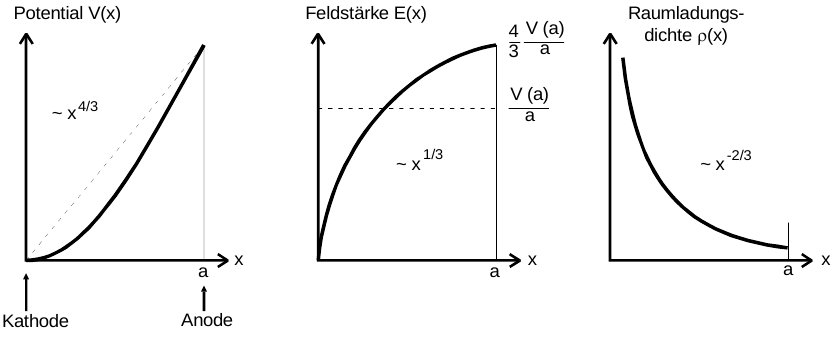
\includegraphics[width=0.8\textwidth]{pics/raumladungsgebiet.jpg}
\label{raumladungsgebiet}
\end{figure}

Den genauen Zusammenhang stellt das Langmuir-Schottkysche Raumladungsgesetz dar:
\begin{equation}
j=\frac{4}{9}\epsilon_0 \sqrt{2e_0/m_0} \frac{V^\frac{3}{2}}{a^2}.
\label{eqlang}
\end{equation}
Eigentlich müsste nach Gleichung \eqref{eqlang} für V=0 auch j=0 gelten, aber dennoch kann man auch ohne angelegtes Potential einen Strom messen. Dieser rührt daher, dass  die Elektronen bereits über einen gewissen Betrag an kinetischer Energie verfügen, wenn sie die Kathode verlassen. Dieser ist sogar groß genug, um gegen ein schwaches Gegenfeld anzulaufen. Entsprechend wird dieser Strom auch Anlaufstrom genannt.\\
In diesem Zusammenhang ist für diesen Versuch insbesondere die sog. Kennlinie der Hochvakuums-Diode interessant. Sie beschreibt den Verlauf des Anodenstroms in Abhängigkeit vom angelegten Potential und lässt sich in drei Bereiche gliedern:  Anlaufstrom-, Raumladungs- und Sättigungsstromgebiet.
\begin{figure}[H]
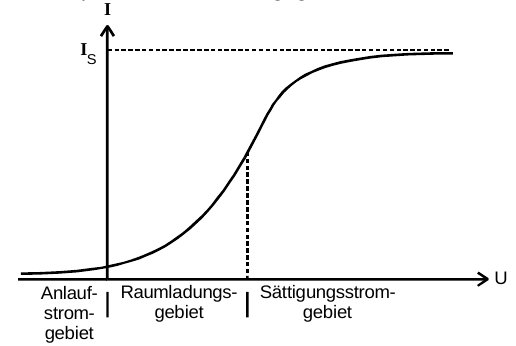
\includegraphics[width=0.479\textwidth]{pics/kennlinie.jpg}
\caption{Glüh-Kathoden-Kennlinie - der Versuchsanleitung entnommen}
\label{pic_kennlinie}
\end{figure}
Im Anlaufstromgebiet zeigt sich, wie viel Kinetische Energie die Elektronen bereits im Metall haben, indem man den Strom misst, der trotz eines Gegenfeldes fließt. Direkt im Anschluss daran findet sich das Raumladungsgebiet. Während die Stärke des angelegten elektrischen Feldes langsam zu Gunsten der Elektronen erhöht wird, gelingt es mehr und mehr von ihnen das Gegenfeld, dass durch die übrigen Elektronen im Raum zwischen Kathode und Anode erzeugt wird, zu überwinden. In Folge dessen steigt der fließende Strom weiter an, bis schließlich im Sättigungsgebiet eine Asymptotische Annährung an einen Maximalwert stattfindet. Dieser Maximalwert entspricht dem Zustand, dass alle Elektronen, die aus der Kathode austreten, zur Anode gelangen. Da die Anzahl der austretenden Elektronen zwar von der Temperatur der Kathode aber nicht von der Stärke des angelegten Feldes abhängt, wird dieser Wert bei einer endlichen Spannung erreicht. 

\subsection{Temperatur}
Den Zusammenhang zwischen angelegter Heizleistung $I_f U_f$ und der resultierenden Kathodentemperatur kann man folgender Gleichung entnehmen.

\begin{formel}
\begin{equation}
I_f U_f = f \eta \sigma T^4 + N_{WL}
\label{eq_temperatur}
\end{equation}
\caption*{\small{$\eta$ = Emissionsgrad der Oberfläche, $\sigma$ =  Stefan-Boltzmann-Konstante, $N_{WL}$ = Wärmeleitung}}
\end{formel}

\subsection{Versuchsaufbau}
Damit die Elektronen nicht sofort mit den umgebenen Luftmolekülen wechselwirken, muss der Versuch im Vakuum durchgeführt werden. Die im Versuch benutzte Apparatur ist eine sog. Hochvakuum-Diode. Sie besteht aus einem evakuierten Glaskolben, in den auf zwei gegenüberliegende Seiten je ein Draht hineinragen.
\begin{figure}[H]
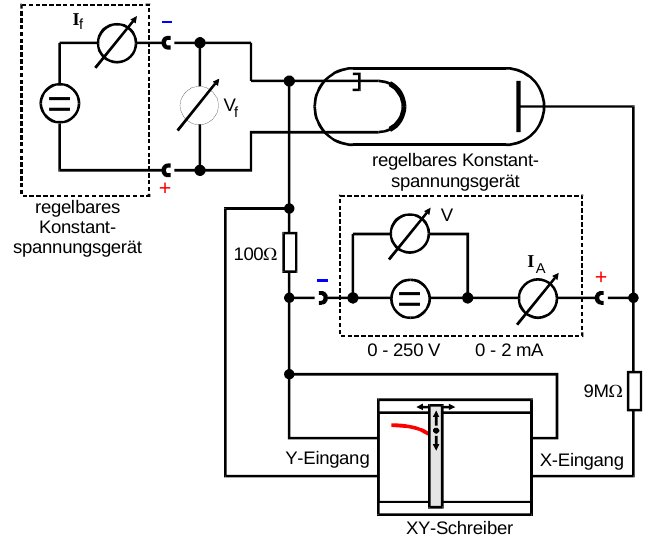
\includegraphics[width=0.5\textwidth]{pics/aufbau1.jpg}
\caption{Für den Versuch verwandter Aufbau - der Versuchsanleitung entnommen}
\end{figure}
Zwischen den Drähten wird später eine Spannung angelegt, so dass die aus der Kathode austretenden Elektronen zur Anode hin beschleunigt werden können. Um die Anzahl an ausgetretenen Elektronen zu erhöhen, wird die Kathode zudem von einem Strom durchflossen, der sie auf 1000 K bis 3000 K erhitzen kann. Die Elektronen treffen schließlich auf die Anode auf und fließen über ein Amperemeter wieder zur Kathode ab.

\section{Durchführung}
\subsection{Kennlinie aufnehmen}
Zunächst sollen für fünf Heizströme die Kennlinien aufgezeichnet werden. Hierzu wird  bei einer gewählten Heizstromstärke die Beschleunigungsspannung des elektrischen Feldes langsam erhöht und die gemessene Stromstärke gegen die angelegte Spannung in einem Diagramm aufgetragen. Es sollten sich dann ein Kurvenverlauf nach Abbildung \ref{pic_kennlinie} ergeben. Anschließend wird nach Möglichkeit der Sättigungsstrom $I_s$ abgelesen.
\subsection{Maximale Heizleistung}
In einem Durchgang wird die maximal erreichbare Heizleistung eingestellt, um das Anlaufstromgebiet zu untersuchen. Es wird hierzu entsprechend des zweiten Schaltbildes ein Gegenfeld aufgebaut und der gemessene Strom gegen die negative Spannung aufgetragen.
\begin{figure}[H]
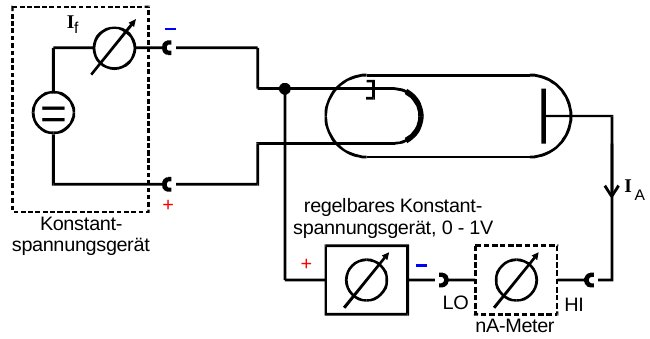
\includegraphics[width=0.5\textwidth]{pics/aufbau2.jpg}
\caption{Schaltbild für Anlaufstromgebiet - der Versuchsanleitung entnommen}
\end{figure}

Außerdem soll der Gültigkeitsbereich für das Langmuir-Schottkysche Raumladungsgesetz gefunden und der Exponent der Strom-Spannungs-Beziehung berechnet werden.
\subsection{Sonstiges}
Zum Schluss sollen noch aus der Leistungsbilanz des Heizstromkreises mittels Gleichung \eqref{eq_temperatur} die Temperatur der Kathode bestimmt werden und mittels der abgelesenen Werte für den Sättigungsstrom $I_s$ soll versucht werden, die Austrittsarbeit des Kathodenmaterials (Wolfram) zu bestimmen.

\section{Auswertung}
\subsection{Fehlerrechnung}
Da viele für die Auswertung notwendigen Größen fehlerbehaftet sind, ist es wichtig, den Einfluss dieser Fehler auf die ermittelten
Größen herauszufinden. Neben den, von den Messapparaturen verursachten Fehlern, dienen der Mittelwert
\begin{formel}
\begin{equation}
 \bar{x} = \frac1N \sum_{i=1}^{N} x_i,
\end{equation}
\caption*{\small{$\bar{x}$ = Mittelwert, N = Anzahl der Messungen}}
\end{formel}

die Gaußsche Fehlerfortpflanzung

\begin{formel}
\begin{equation}
\Delta G = \sqrt{\sum_{i=1}^{N}\left( \frac{\partial G}{\partial x_i}\cdot \Delta x_i\right)^2},
\label{gauss}
\end{equation}
\caption*{$x_i$ = Variable, $\Delta x_i$ = Fehler der Variable}
\end{formel}

und die Standardabweichung des Mittelwerts

\begin{equation}
 \bar s = \sqrt{\frac{1}{N(N-1)} \sum_{i}^{N} (x_i - \bar{x})^2}.
\end{equation}

\subsection{Kennlinienschar der Hochvakuumdiode}
\label{a}
Unter Anlegung von fünf verschiedenen Heizströmen $I_f$ wird die Beschleunigungsspannung $U_A$ erhöht und der fließende Strom $I_A$ 
gemessen. Ab einem gewissen Strom $I_S$ hat die Beschleunigungsspannung keinen Einfluss mehr auf die weitere Steigung. Man spricht vom
Sättigungsstrom.

In Abbildung \ref{picheiz} sind die Wertepaare visualisiert. Bei den ersten vier Heizströmen ist der Sättigungsstrom gut abschätzbar.
Beim fünften wurde das Steigungsverhalten betrachtet und der zugehörige Schwellenwert abgeschätzt. Das Verhalten der Kurvenschar 
entspricht deutlich dem Erwarteten, vergleichbar mit Abbildung \ref{refheiz}.

\renewcommand{\arraystretch}{0.9}
\begin{table}[H]
\begin{tabular}{|c||c|c|c|c|c|}
$U_A$ in V & $I_f$ = 2,2 A  & $I_f$ = 2,4 A  & $I_f$ = 2,5 A  & $I_f$ = 2,6 A  & $I_f$ = 2,8 A\\
 \hline
& $I_A$ in $\mu$A &$I_A$ in $\mu$A &$I_A$ in $\mu$A &$I_A$ in $\mu$A &$I_A$ in $\mu$A \\ 
\hline
1&	&	3&	5&	5&	6\\
2&	3&	7&	8&	9&	13\\
3&	4&	10&	12&	15&	18\\
4&	6&	13&	16&	18&	24\\
5&	7&	16&	20&	24&	29\\
6&	&	19&	24&	28&	35\\
7&	8&	22&	28&	33&	40\\
8&	9&	24&	32&	38&	46\\
9&	&	27&	35&	42&	52\\
10&	10&	30&	40&	48&	57\\
11&	&	&	44&	&	\\
12&	11&	35&	48&	60&	72\\
13&	11&	&	53&	&	\\
14&	&	&	57&	70&	86\\
15&	12&	43&	61&	&	\\
16&	&	&	&	83&	103\\
18&	&	&	&	97&	212\\
20&	14&	54&	84&	110&	139\\
22&	&	&	92&	124&	155\\
24&	&	&	&	138&	172\\
25&	14&	62&	104&	144&	184\\
26&	&	&	&	151&	193\\
27&	&	&	109&	&	\\
28&	&	&		&165&	213\\
30&	15	&68&	120&	177&	233\\
32&	&	&	&	&	255\\
34&	&	&	&	&	276\\
35&	16&	72&	133&	206&	\\
36&	&	&	&	&	297\\
38&	&	&	&	&	320\\
40&	16&	75&	140&	233&	343\\
45&	&	&	146&	252&	405\\
50&	17&	76&	147&	265&	462\\
55&	&	&	&	278&	522\\
60&	&	&	150&	289&	572\\
70&	&	79&	156&	305&	680\\
80&	&	&	160&	316&	785\\
90&	&	83&	167&	325&	872\\
100&	19&	85&	166&	332&	937\\
110&	&	&	&	&	980\\
120&	&	&	&	&	1010\\
125&	19&	&	&	&	\\
130	&	&	&	&	&1040\\
140&	&	&	&		&1060\\
150&	&	87&	170&	336&	1080\\
200&	&	&	&	&	1130\\
\hline
\textbf{$I_S$} & \textbf{20} & \textbf{89} & \textbf{172} & \textbf{338} & \textbf{1190} \\
\hline
\end{tabular}
\caption{Beschleunigungsspannung $U_A$ und Strom $I_A$ zu fünf Heizströmen $I_f$, sowie die Sättigungsströme $I_S$}
\label{tabheiz}
\end{table}
\renewcommand{\arraystretch}{1}


\begin{figure}[H]
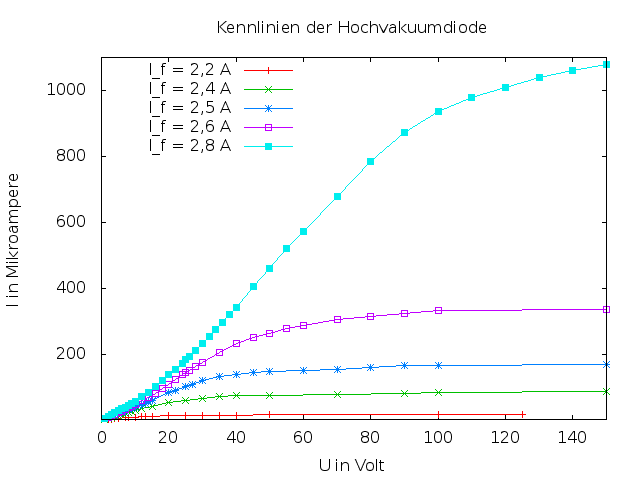
\includegraphics[width=0.8\textwidth]{pics/504a.png}
\caption{Wertepaare aus Tabelle \ref{tabheiz}}
\label{picheiz}
\end{figure}

\subsection{Langmuir-Schottky Exponent}
\label{expo}
Nach Gleichung \eqref{eqlang} wird eine $\sqrt{V^3}$-Abhängigkeit zwischen Stromdichte $j$ und der Anodenspannung $U_A$ erwartet. Unter
Betrachtung des höchsten Heizstroms $I_f$ = 3,0 A wird das Verhalten beobachtet. In Tabelle \ref{tablang} werden die ensprechenden Wertepaare
aufgeführt und in Abbildung \ref{piclang} dargestellt. Der Fehler $\Delta U$ ergibt sich aus der Angabe des Messgeräts durch 1,5\% seines
Vollausschlags mit 60 V bzw. 100 V. 

\begin{table}[H]
\begin{tabular}{|c|c|c|c|c|}
$U_A$ in V & $I_A$ in $\mu$A & $\ln(U/V)$ & $\ln(I/\mu A)$ & $\Delta U$ in V\\
\hline
5&	38&	1,61&	3,64&0,9 \\
10&	70&	2,30&	4,25&0,9\\
15&	113&	2,71&	4,73&0,9\\
20&	160&	3,00&	5,08&0,9\\
25&	210&	3,22&	5,35&0,9\\
30&	270&	3,40&	5,60&0,9\\
35&	336&	3,56&	5,82&0,9\\
40&	396&	3,69&	5,98&0,9\\
45&	468&	3,81&	6,15&0,9\\
50&	543&	3,91&	6,30&0,9\\
55&	623&	4,01&	6,43&0,9\\
60&	695&	4,09&	6,54&3,75\\
70&	893&	4,25&	6,79&3,75\\
80&	1070&	4,38&	6,98&3,75\\
90&	1240&	4,50&	7,12&3,75\\
\hline
\end{tabular}
\caption{Beschleunigungsspannung $U_A$ und Strom $I_A$ bei einem Heizstrom $I_f$ = 3,0 A}
\label{tablang}
\end{table}

Mittels linearer Regression von GNUplot durchgeführt, ergibt sich nach reduzierter Gleichung \eqref{eqlang} 

\begin{align}
 \ln(j) \propto a \cdot \ln(V) \intertext{ein Exponent von}
 a = 1,247 \pm 0,03.
\end{align}

Durch einen Fit ensprechend der normalen Form von Gleichung \eqref{eqlang} war ein besserer Wert für den Exponenten feststellbar

\begin{align}
 a = 1,39 \pm 0,05.
\end{align}


\begin{figure}[H]
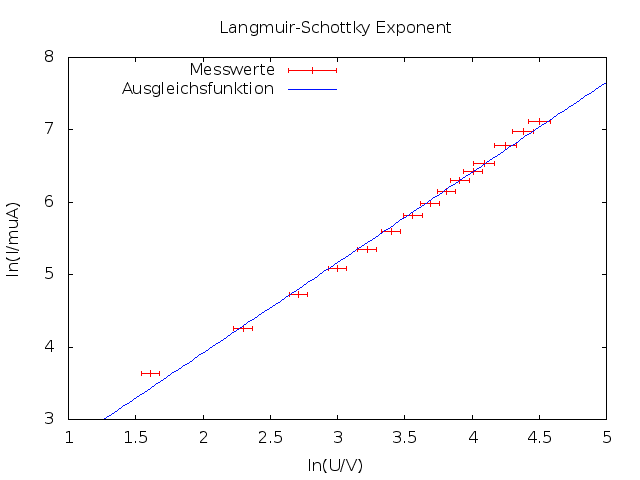
\includegraphics[width=0.8\textwidth]{pics/504b2.png} 
\caption{doppellogarithmische Auftragung von $I_A$ und $U_A$ bei einem Heizstrom von $I_f$ = 3,0 A. Die Steigung entspricht dem Exponenten}
\label{piclang}
\end{figure}
\begin{figure}[H]
 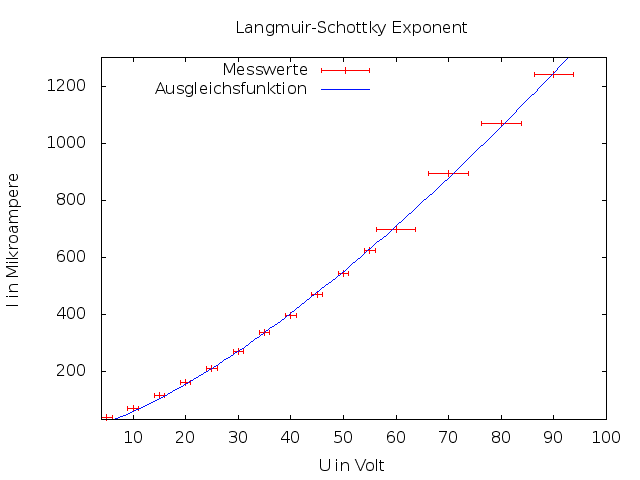
\includegraphics[width=0.8\textwidth]{pics/504b1.png} 
 \caption{Darstellung der $\sqrt{V^3}$-Abhängigkeit zwischen Stromdichte $j$ und Anodenspannung $U_A$}
\end{figure}

\subsection{Kathodentemperatur}
\label{kath}
Die Stromdichte $j(V)$ hängt im Bereich des Anlaufstromgebiets zudem von der Temperatur der Kathode nach Gleichung \eqref{eqtemp} ab.
Durch die gemessene Anodenspannung, sowie den Anodenstrom lässt sich somit die Kathodentemperatur $T$ ermitteln. Da die Anodenspannung
für ein Gegenfeld benötigt wird, ist $V_A$ negativ. Die Korrektur der Spannung muss aufgrund des Spannungsabfalls am Nanoamperemeter
durchgeführt werden, welcher einen Innenwiderstand von $R_i$ = 1M$\Omega$ aufweist.

\begin{table}[H]
\begin{tabular}{|c|c|c|c|c|c|}
$U_{mess}$ in V & $U_{korr}$ in V & $I_{mess}$ in nA & $\ln(I_{mess}/nA)$ & $\Delta U$ in V & $\Delta I$ in nA \\
\hline
0&	0,255&	255&	5,541&	0,02&	0,06 \\
-0,1&	0,295&	195&	5,273&	0,02&	0,06\\
-0,2&	0,350&	150&	5,011&	0,02&	0,06\\
-0,3&	0,410&	110&	4,700&	0,02&	0,06\\
-0,4&	0,478&	78&	4,357&	0,02&	0,06\\
-0,5&	0,553&	53&	3,970&	0,02&	0,06\\
-0,6&	0,631&	31&	3,434&	0,02&	0,06\\
-0,7&	0,721&	21&	3,045&	0,02&	0,06\\
-0,8&	0,813&	13&	2,565&	0,02&	0,06\\
-0,9&	0,908&	7,5&	2,015&	0,02&	0,06\\
-0,93&	0,936&	5,5&	1,705&	0,02&	0,06\\
\hline
\end{tabular}
\caption{$U_A$ gegen $I_A$ zur Ermittlung der Kathodentemperatur}
\label{tabtemp}
\end{table}

Von GNUplot wird die reduzierte Gleichung \eqref{eqtemp}

\begin{align}
 T = \frac{e_0}{k_B \, b}
\end{align}

mit den Messwerten aus Tabelle \ref{tabtemp} gefittet, was zum Koeffizienten $b$ mit

\begin{align}
 b = (-5,463 \pm 0,079) \, \frac{1}{V}
\end{align}

führt und damit zu einer Kathodentemperatur von

\begin{align}
 T = (2125 \pm 1,1)\, K.
\end{align}

\begin{figure}[H]
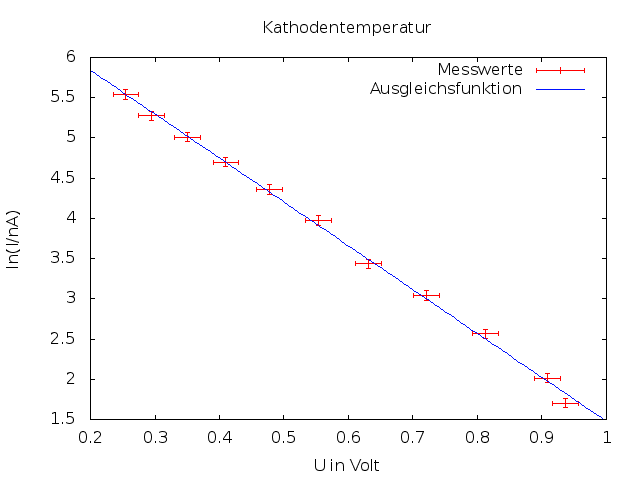
\includegraphics[width=0.8\textwidth]{pics/504c.png}
\caption{Abhängigkeit von $U$ und $\ln(I)$ im Anlaufstromgebiet zur Ermittlung des Koeffizienten $b$}
\end{figure}

Die Kathodentemperatur lässt sich im Bereich des Raumladungsgebiets aus einer Leistungsbilanz herausrechnen. Hierzu werden die Heizleistungen,
die in Abschnitt \ref{a} aufgeführt sind verwenden und nach folgender Gleichung die Kathodentemperatur ermittelt.

\begin{formel}
 \begin{align}
  T = \sqrt[4]{\frac{I_f\,U_f - N_{WL}}{f \, \eta \, \sigma}}
 \end{align}
\caption*{\small{$N_{WL}$ = Wärmeleitung, $f$ = Kathodenoberfläche, $\eta$ = Emissionsgrad, $\sigma$ = Stefan-Boltzmann Konstante}}
\end{formel}


\begin{table}[H]
 \begin{tabular}{c|c|c}
  $I_f$ & $U_f$ & $T_K$ \\
  \hline
2,2&	3,20&	1813 \\
2,4&	3,72&	1940\\
2,5&	4,01&	2004\\
2,6&	4,30&	2066\\
2,8&	4,89&	2183\\
 \end{tabular}
\caption{Kathodentemperatur $T_K$ errechnet aus der Heizleistungsbilanz}
\end{table}

\subsection{Austrittsarbeit des Kathodenmaterials Wolfram}
\label{wolf}
Um nun die Austrittsarbeit zu errechnen, wird die Richardson-Gleichung \eqref{eqrich} nach  $\Phi$ umgestellt. Die $I_S$-$T_K$-Wertepaare,
die in den Abschnitten \ref{a} und \ref{kath} ermittelt wurden, werden ensprechend eingesetzt.

\begin{align}
 \Phi = \frac{k_B \, T}{e_0} \cdot \ln\left(\frac{I_S}{T_K^2}A \right) \quad \text{mit} \quad A = \frac{h^3}{4 \pi \, f \, e_0 \, m_0 \, k^2}
\end{align}

\begin{table}[H]
 \begin{tabular}{c|c|c|c}
$I_f$ in A & $I_S$ in $\mu$A & $T_K$ in K &$\Phi$ in eV \\
\hline
2,2&	19		&	1813&	4,62\\
2,4&	88		&	1940&	4,72\\
2,5&	170		&	2004&	4,77\\
2,6&	336		&	2066&	4,81\\
2,8&	1190	&	2183&	4,86 \\

 \end{tabular}
\caption{Austrittsarbeiten $\Phi$ zu den verschiedenen Kathodentemperaturen und den Sättigungsströmen}
\label{tabrich}
\end{table}

Aus den in Tabelle \ref{tabrich} angegebenen Austrittsarbeiten ergibt sich der Mittelwert zu

\begin{equation}
 \bar \Phi = (4,755 \pm 0,006)\, \text{eV}
\end{equation}

\section{Diskussion}
Der in Abschnitt \ref{expo} ermittelte Wert für den Langmuir-Schottky Exponenten mit einem Wert von 

\begin{equation*}
 a = 1,241 \pm 0,03 \quad \text{bzw.} \quad 1,39 \pm 0,05
\end{equation*}

liegt nahe bei dem erwarteten Wert von 1,5 mit einem Fehler von 17,3 \% bzw. 7,4 \%. 

Die in \ref{kath} ermittelte Kathodentemperatur, welche zu einem Heizstrom von 3,0 A gehört, bewegt sich in derselben Größenordnung,
wie die im selben Abschnitt errechnete Kathodentemperatur bei 2,8 A

\begin{equation*}
 T = (2125 \pm 1,1)\, K \quad \text{und} \quad T_{K,2,8} = 2183 \, K
\end{equation*}

Und schließlich die Austrittsarbeit von Wolfram, errechnet in Abschnitt \ref{wolf}, mit einem Wert von 

\begin{equation*}
 \Phi = (4,755 \pm 0,006) \, \text{eV}
\end{equation*}

hat eine Abweichung von 4,5 \% zum Referenzwert
\footnote[1]{Adeos Media GmbH (2004), URL: \href{http://www.formel-sammlung.de/formel-Austrittsarbeit-von-Elektronen-aus-Metallen-3-25-134.html}{www.formel-sammlung.de}}




% ========================================
%	Literaturverzeichnis
% ========================================

%\bibliographystyle{plainnat}			% Bibliographie-Style auswählen
%\bibliography{BIBDATEI}			% Literaturverzeichnis

% ========================================
%	Das Dokument endent
% ========================================

\end{document}
